%-------------------------------------------------------------------------------
%                            BAB III
%               		METODOLOGI PENELITIAN
%-------------------------------------------------------------------------------
\fancyhf{} 
\fancyfoot[C]{\thepage}
\chapter{METODOLOGI PENELITIAN}

\section{\uppercase{WAKTU DAN LOKASI PENELITIAN}}
\setlength\parindent{30pt} Penelitian ini dilaksanakan di Ruang Kuliah B.03.02 yang terletak di lantai 3 Blok B dan Ruang Kuliah E.02.07 yang terletak di lantai 2 Blok E, Gedung FMIPA Universitas Syiah Kuala (Unsyiah). Waktu yang dibutuhkan untuk penelitian ini adalah 6 bulan terhitung dari bulan Juli 2019 hingga Februari 2020. 

\section{\uppercase{ALAT DAN BAHAN}}
Alat dan bahan yang digunakan pada penelitian ini meliputi perangkat keras, perangkat lunak dan bahan yang mendukung pada penelitian ini adalah data \textit{Received Signal Strength Indicator} (RSSI) dari hasil survei di lokasi penelitian. Perangkat lunak yang digunakan adalah:
\begin{itemize}
\itemsep0em
\item OS Windows 10.
\item Android Studio 3.6.
\item IntelliJ IDEA 2019.3.3.
\item PhpStorm 2019.3.3.
\item Postman 7.19.1.
\end{itemize}

\par Sedangkan komponen perangkat keras yang digunakan meliputi 1 unit Laptop Lenovo dengan RAM 6GB, Intel® Core™ i5-3230M CPU @2.60Ghz (4 CPUs), ~2.6 GHz Processor, \textit{Harddisk} 500GB, \textit{Solid State Drive} (SSD) 120GB, memiliki Sistem Operasi Windows 64-bit, 3 unit Nyvida Beacon, dan 6 unit FeasyBeacon. 

\section{\uppercase{METODE PENELITIAN}}
Metode penelitian yang dilakukan terdiri dari beberapa tahapan. Skema dari alur tahapan tersebut dapat dilihat pada Gambar \ref{metpen}.
\begin{figure}[H]
\centering
{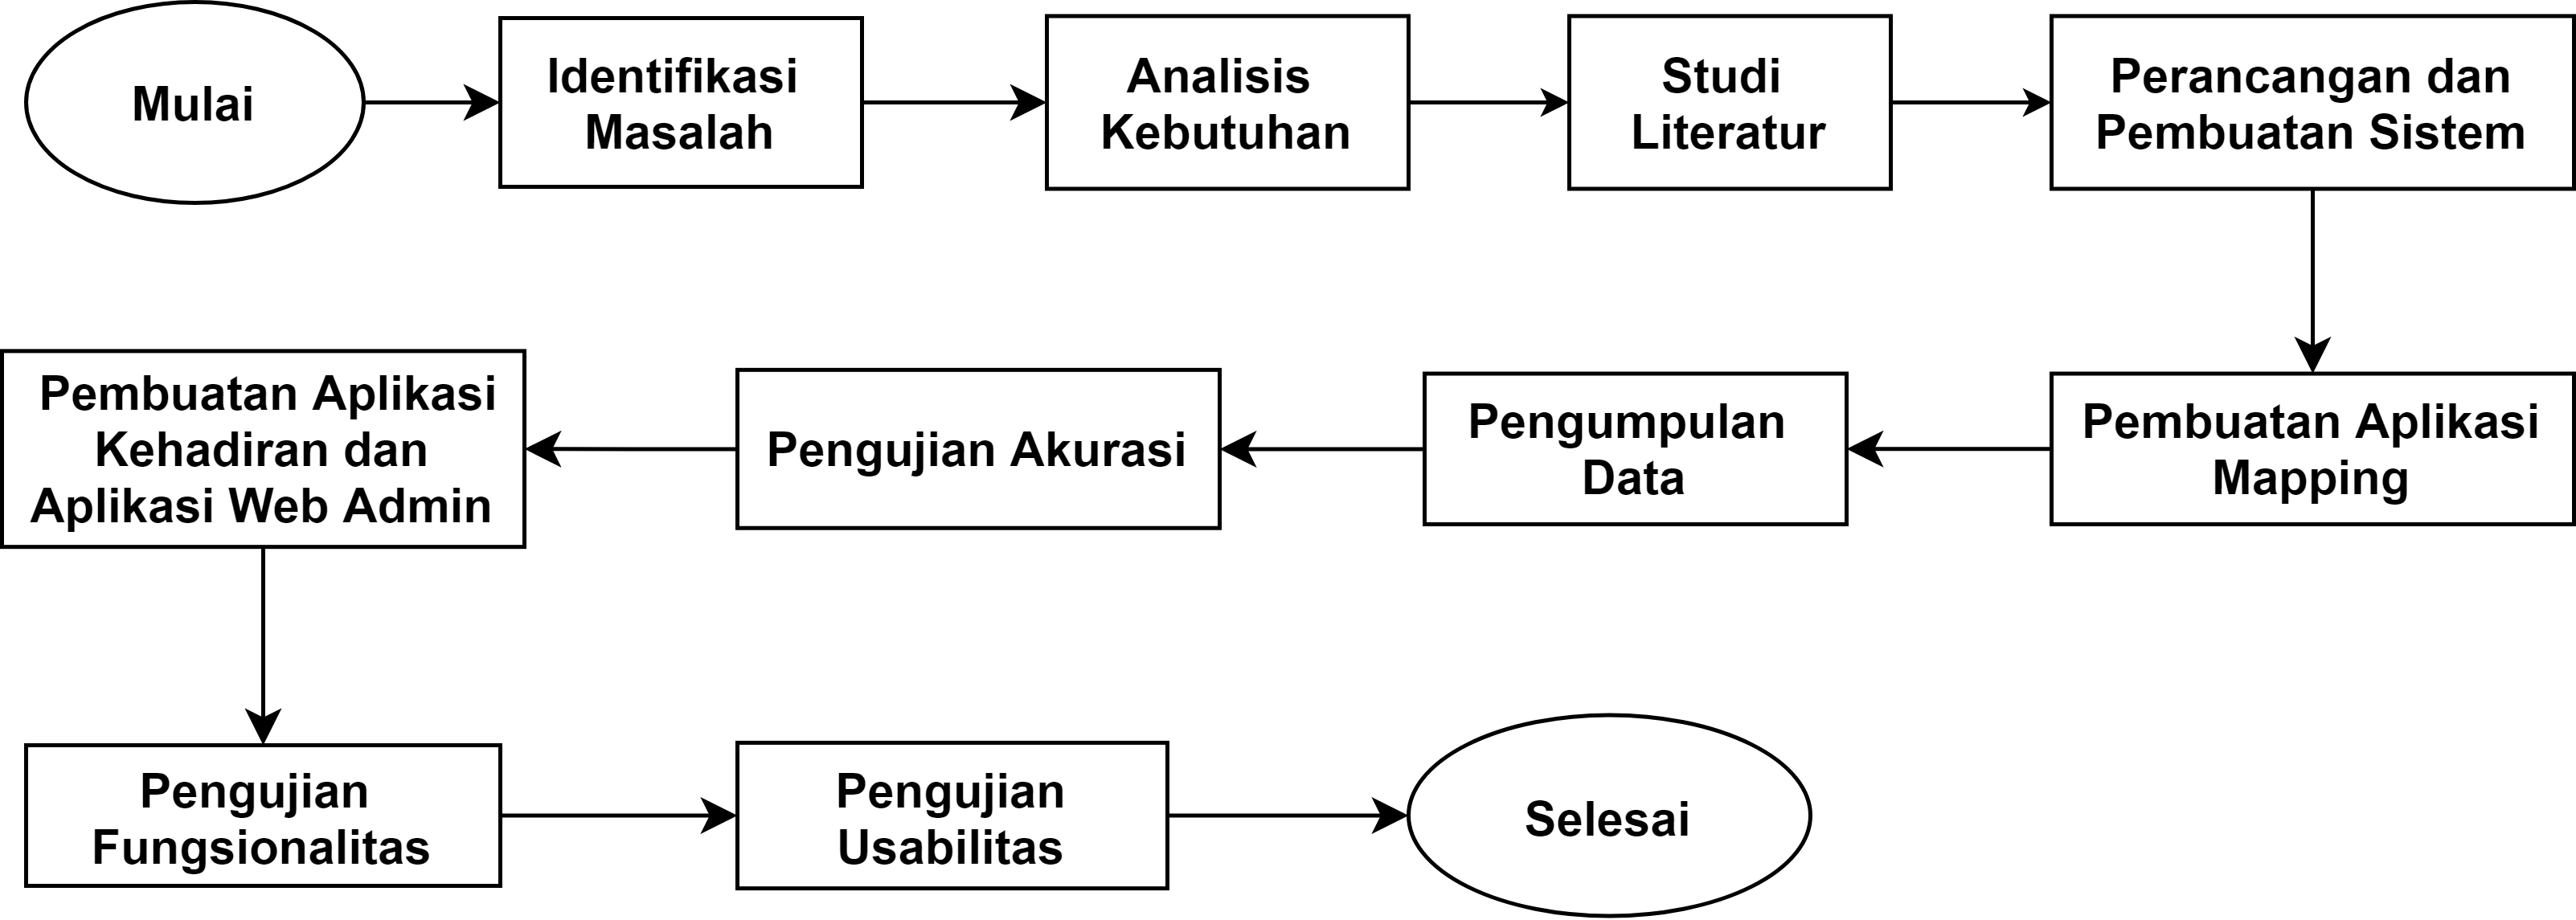
\includegraphics [width = 14cm, height= 6cm]{gambar/diagram-alir-penelitian}}
\caption{Diagram Alir Penelitian}
\label{metpen}
\end{figure}

\fancyhf{} 
\fancyfoot[R]{\thepage}

\subsection{Identifikasi Masalah}
Tahapan ini merupakan tahapan yang dilakukan untuk mengidentifikasi masalah sehingga aplikasi ini perlu dibuat. Masalah-masalah yang berhasil diidentifikasi adalah sebagai berikut:
\begin{enumerate}[1.]
\itemsep0em
\item Belum tersedia Aplikasi Mapping untuk pemetaan kekuatan sinyal atau pemetaan nilai RSSI berbasis Android. 
\item Teknologi GPS tidak berfungsi dengan baik apabila digunakan di dalam gedung \citep{Keluza2017}.
\item Belum tersedia Aplikasi Kehadiran berbasis Android di Jurusan Informatika Unsyiah.
\end{enumerate}

%%%%%%%%%%%%%%%%%%%%%%%%%%%%%%%%%%%%%%%%%%%
\subsection{Analisis Kebutuhan}
Tahapan ini dilakukan untuk mengetahui kebutuhan yang bersumber dari masalah yang telah diidentifikasi sebelumnya sehingga perancangan aplikasi dibangun sesuai kebutuhan. Kebutuhan dari sistem yang dibangun adalah sebagai berikut:

\par \textbf{Kebutuhan Fungsional} Kebutuhan fungsional mendefinisikan fungsionalitas sistem. Kebutuhan fungsional dari identifikasi masalah yang telah dilakukan adalah sebagai berikut:

\begin{itemize}
\item Melakukan proses pencatatan kehadiran dosen dan mahasiswa secara \textit{background proccess} dengan aplikasi berbasis Android dengan akurasi yang baik apabila di dalam gedung.

\item Menampilkan prediksi lokasi pengguna.

\end{itemize}

\par \textbf{Kebutuhan Non-Fungsional} Kebutuhan non-fungsional memastikan batasan eksternal yang harus dipenuhi oleh sistem. Batasan-batasan tersebut antara lain:
\begin{itemize}
\item Proses pencatatan kehadiran perkuliahan dimulai oleh dosen.

\item Dosen dan mahasiswa tidak dapat melakukan proses pencatatan kehadiran apabila terlambat 50 menit sebelum perkuliahan berakhir.

\item Proses pencatatan kehadiran dilakukan secara \textit{background proccess} dengan menit yang diacak setiap rentang waktu 10 menit.

\item Hanya dapat melakukan proses pencatatan kehadiran apabila Bluetooth pada perangkat hidup dan terkoneksi dengan internet.

\item Sistem hanya dapat mendeteksi lokasi pengguna di dalam gedung yang telah dipetakan terlebih dahulu.
 
\end{itemize}

%%%%%%%%%%%%%%%%%%%%%%%%%%%%%%%%%%%%%%%%%
\subsection{Studi Literatur}
Studi literatur digunakan sebagai bahan referensi selama proses penelitian. Studi literatur dilakukan dengan cara mencari situs \textit{website} dan jurnal-jurnal terkait tentang penelitian, baik jurnal nasional maupun jurnal internasional, buku-buku yang telah diterbitkan, serta situs-situs internet yang berkaitan dengan permasalahan yang dikaji dalam penelitian. Studi literatur dapat dikembangkan untuk menyempurnakan kekurangan dari penelitian sebelumnya. 

\subsection{Perancangan Sistem dan Pembuatan Sistem}
\subsection{Perancangan Sistem}
Tahap perancangan sistem ini meliputi perancangan alur kerja sistem yang berfungsi untuk memastikan sistem yang dibangun dapat digunakan secara baik oleh pengguna. Alur kerja dari sistem yang dibangun dijelaskan dengan menggunakan diagram alir yang dapat dilihat pada Gambar \ref{alur-kerja-sistem}.

\begin{figure}[H]
\centering
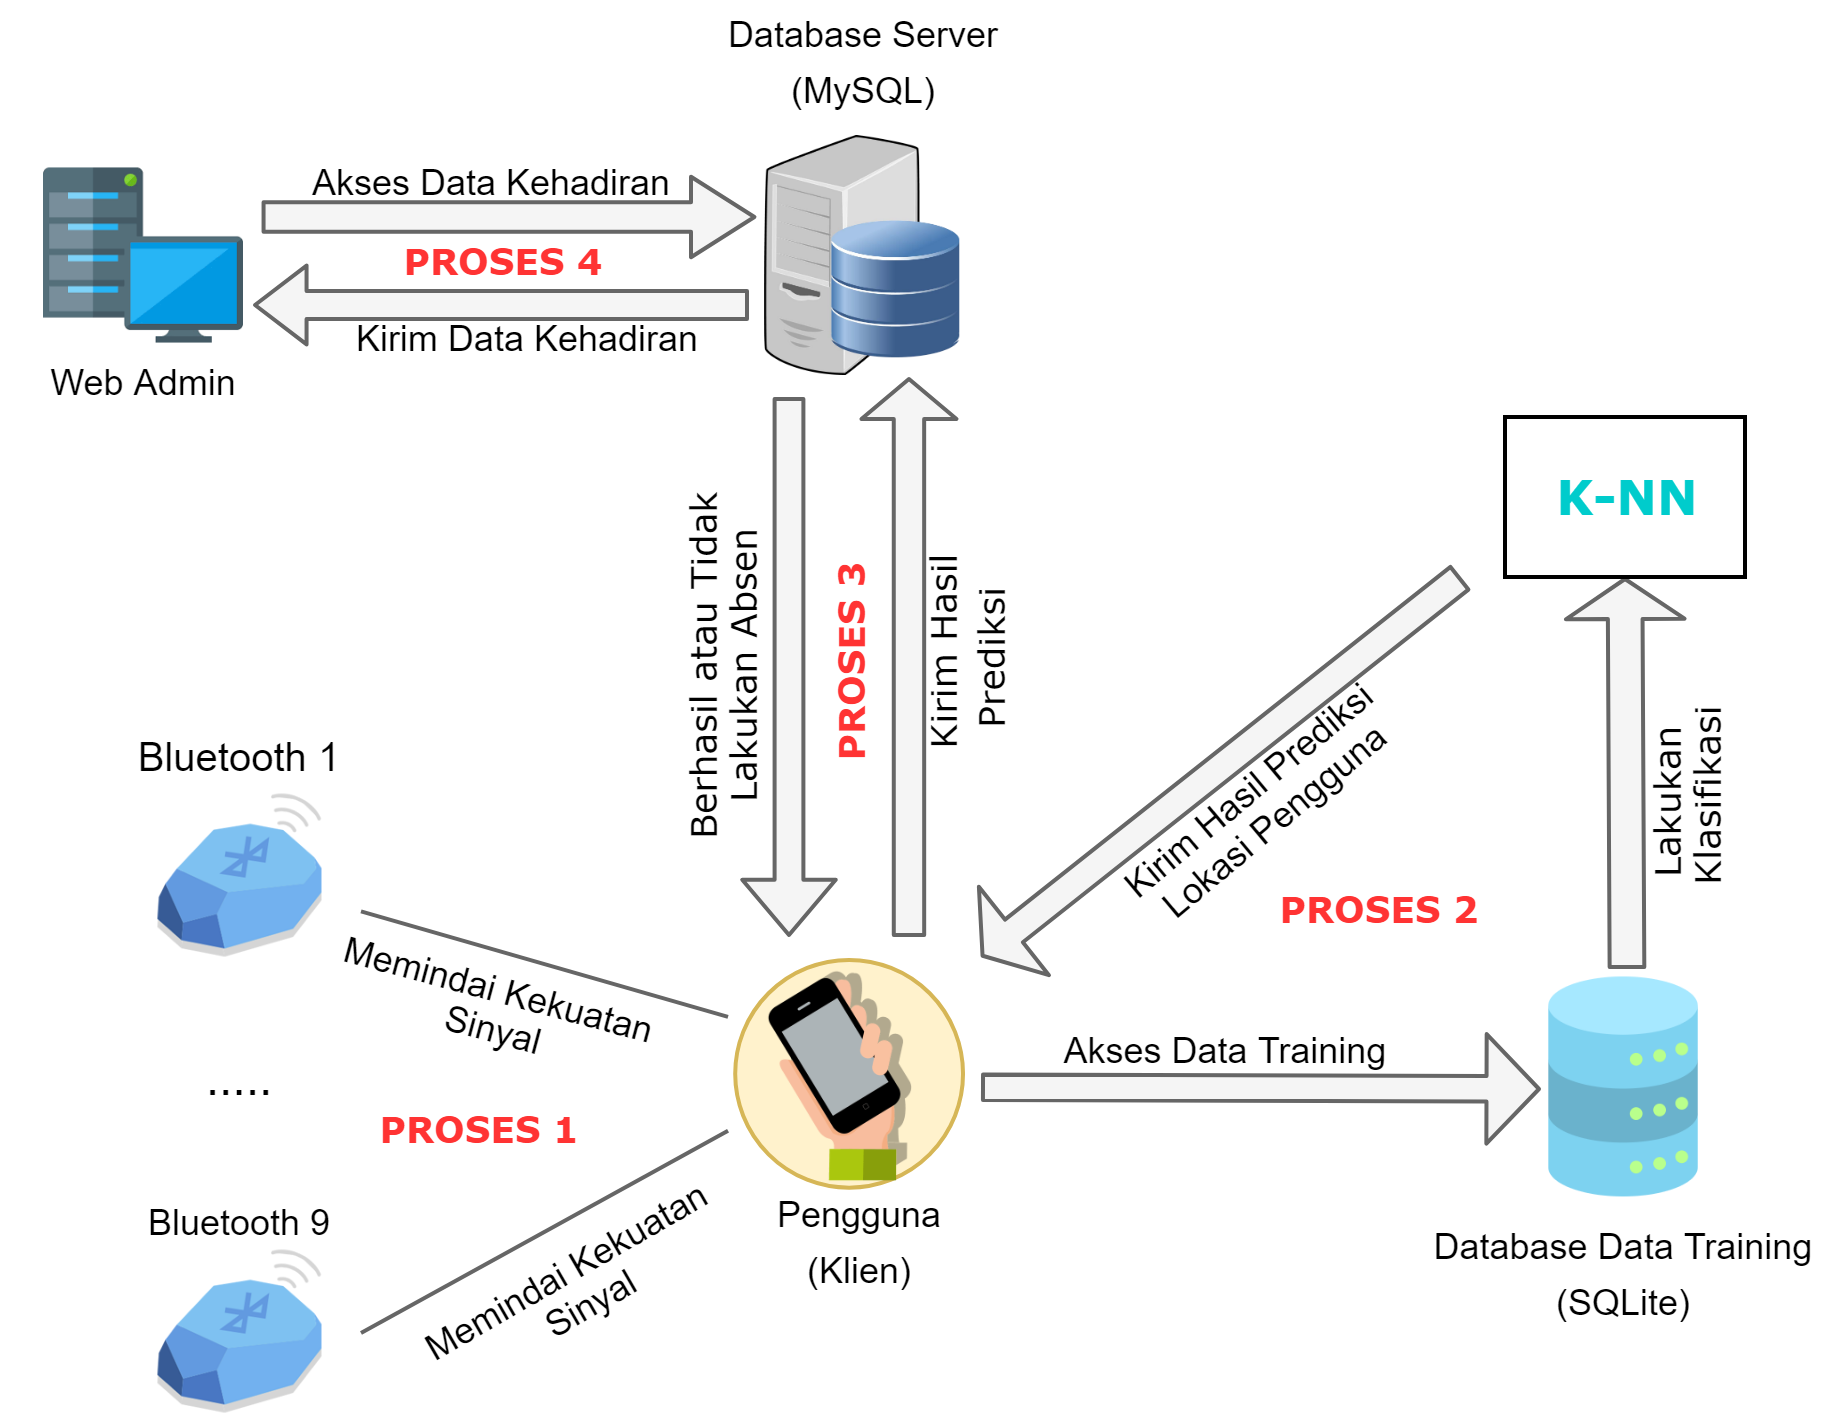
\includegraphics[width=10cm, height=8cm]{gambar/alur-kerja-aplikasi}
\caption{Alur Kerja Sistem.}
\label{alur-kerja-sistem}
\end{figure}

\subsection{Pembuatan Sistem}
Pada proses pembuatan sistem, metode pengembangan perangkat lunak yang digunakan yaitu metode \textit{Scrum}, dikarenakan sistem ini dikembangkan dengan bekerja secara tim dan membutuhkan fleksibilitas terhadap perubahan yang terjadi dalam proses pengembangannya, sehingga memerlukan iterasi secara berkala agar berjalan dengan baik. Sistem ini memiliki empat aplikasi yang terdiri dari tiga aplikasi utama dan satu aplikasi pendukung. yaitu:
\begin{enumerate}
\item Aplikasi Mapping 
\newline Aplikasi ini merupakan aplikasi pendukung yang berfungsi untuk melakukan pengumpulan data. Data yang dikumpulkan berupa data kekuatan sinyal berdasarkan lokasi dimana data tersebut diambil. Setelah pengumpulan data selesai dilakukan, data tersebut ditanamkan kedalam aplikasi Kehadiran Dosen dan aplikasi Kehadiran Mahasiswa.

\item Aplikasi Kehadiran Dosen
\newline Aplikasi ini merupakan aplikasi utama yang berfungsi untuk melakukan proses pencatatan kehadiran dosen secara \textit{background proccess} dan memprediksi lokasi dosen apakah sesuai dengan kelas dimana proses perkuliahan tersebut berlangsung.

\item Aplikasi Kehadiran Mahasiswa
\newline Aplikasi ini merupakan aplikasi utama yang berfungsi untuk melakukan proses pencatatan kehadiran mahasiswa secara \textit{background proccess} dan memprediksi lokasi mahasiswa apakah sesuai dengan kelas dimana proses perkuliahan tersebut berlangsung.

\item Aplikasi Web Admin
\newline Aplikasi ini merupakan aplikasi utama yang berfungsi untuk melihat dan mengunduh data kehadiran dosen dan mahasiswa sebagai \textit{back-up}.
\end{enumerate}

\subsection{Pembuatan Aplikasi Mapping}
\par Aplikasi ini merupakan aplikasi \textit{mobile} berbasis Android yang berguna untuk penyimpanan kekuatan sinyal atau penyimpanan nilai RSSI pada penelitian ini. Adapun fitur-fitur yang tersedia adalah sebagai berikut:

\begin {itemize}
\itemsep0em
\item Pemindaian Kekuatan Sinyal \newline
Aplikasi dapat melakukan proses pemindaian kekuatan sinyal dari setiap Beacon. Setelah proses pemindaian selesai, aplikasi akan menampilkan informasi setiap Beacon yang terdeteksi seperti: MAC Address, nilai RSSI, dan nama perangkat Beacon tersebut. 

\item Menyimpan Data Kekuatan Sinyal \newline
Ketika aplikasi selesai mendeteksi kekuatan sinyal dari Beacon, kekuatan sinyal tersebut dapat disimpan ke dalam basis data lokal untuk keperluan penelitian pada tahap pengumpulan data.

\item Menampilkan Data Kekuatan Sinyal \newline
Data-data kekuatan sinyal yang tersimpan di basis data aplikasi dapat ditampilkan ke dalam bentuk \textit{list} yang berisi informasi seperti: nama ruang dimana pemindaian kekuatan sinyal dilakukan, MAC Address Beacon, dan nilai RSSI setiap Beacon.

\item Menghapus Data \newline
Aplikasi memiliki fitur untuk menghapus data kekuatan sinyal yang tidak diperlukan. 

\end{itemize}

%%%%%%%%%%%%%%%%%%%%%%%%%%%%%%%%%%%%%%%%%%%%%%%%%%%%%%%%%%%%%%%%%%%%%%%%%%%%%%%%%%%%%%%%%%%%%%%%%%%%%%%%%%%%%%%%%%
\subsection{Pengumpulan Data}
\begin{enumerate}[a.]
\itemsep0em
\item Pembuatan Denah Lokasi Penelitian
\\
Pembuatan denah lokasi penelitian didasarkan pada rancangan gedung yang diperoleh. Denah ini digunakan untuk membantu dalam menentukan letak \textit{reference point} pada proses pemetaan kekuatan sinyal. Proses penentuan letak \textit{reference point} ini dilakukan dengan cara menghitung luas lokasi penelitian.
%%%%%%%%%%%%%%%%%%%%%%next%%%%%%%%%%%%%%%%%%%%%
\\
\\
\item Penentuan Letak \textit{Reference Point}
\\
Penentuan letak \textit{reference point} dilakukan di Ruang Kuliah B.03.02 yang terletak di lantai 3 Blok B dan Ruang Kuliah E.02.07 yang terletak di lantai 2 Blok E, dengan tujuan untuk mendeteksi lokasi pengguna di lantai yang berbeda dengan jarak antar Ruang Kuliah B.03.02 dan Ruang Kuliah E.02.07 yang terletak cukup jauh di dalam gedung FMIPA Unsyiah. Penentuan letak \textit{reference point} ini dilakukan didalam kelas dan diluar kelas, dengan tujuan untuk menguji tingkat keberhasilan klasifikasi ruangan yang berdekatan. Penentuan \textit{reference point} dipetakan secara urut menggunakan koordinat \textit{cartesian} dengan masing-masing jarak antar satu \textit{reference point} ke \textit{reference point} yang lain sejauh 2 meter untuk meminimalisir \textit{position error} \citep{Lee2019} dan secara acak tanpa memperhitungkan jarak antar \textit{reference point} \citep{Bahl2000}. Penentuan letak \textit{reference point} ini bertujuan untuk menentukan lokasi pengambilan data kekuatan sinyal yang dipancarkan setiap Beacon. Penentuan \textit{reference point} yang saling berdekatan mempengaruhi hasil tahap \textit{positioning} \citep{darshan2012}. Denah lokasi penelitian ini dapat dilihat pada Gambar \ref{kelasb0302} dan Gambar \ref{kelase0207}.

\vspace{2cm}
\begin{landscape}
\begin{figure}[H]
    \centering
    \subfloat[Reference Point Urut]{{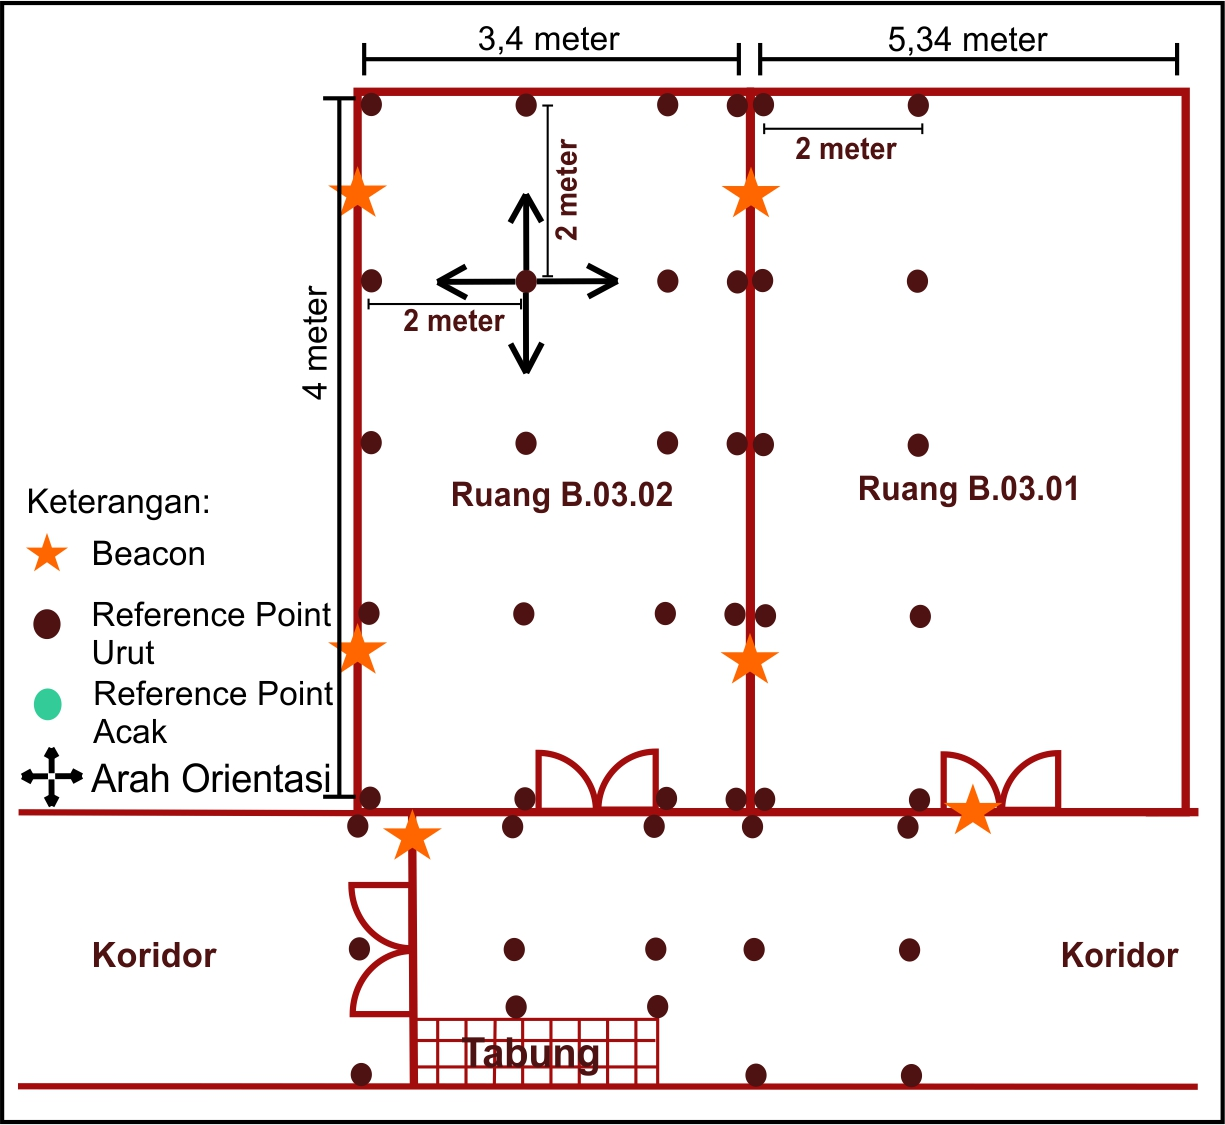
\includegraphics[width=10cm, height=9cm]{gambar/denah/B0302-Urut} }}%
    \qquad
    \subfloat[Reference Point Acak]{{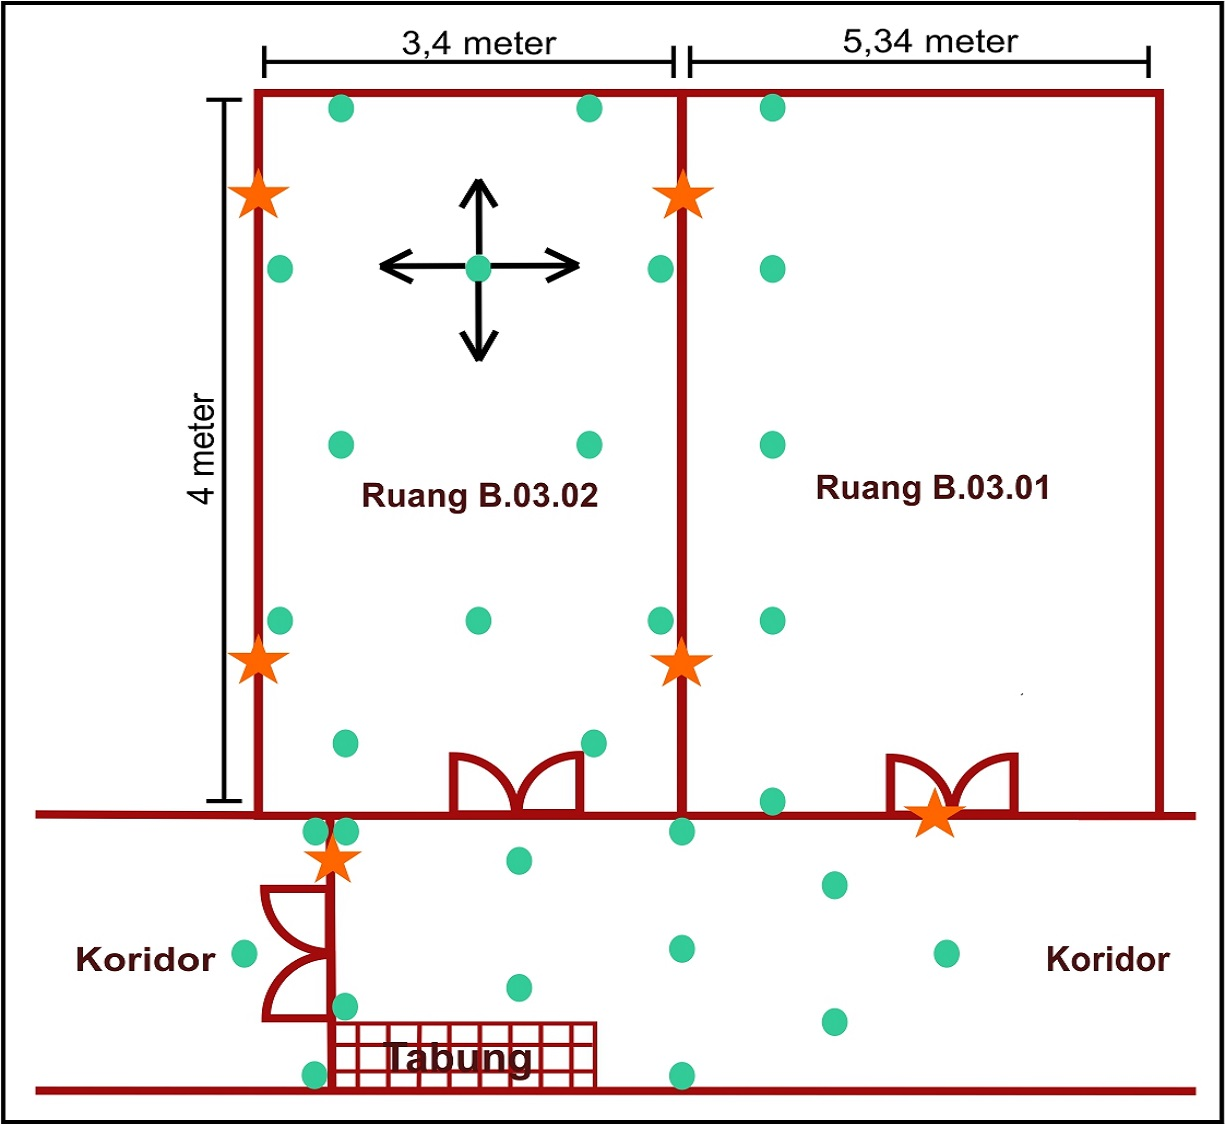
\includegraphics[width=10cm, height=9cm]{gambar/denah/B0302-Acak} }}%
    \caption{Denah Lokasi Penelitian Ruang B.03.02}%
    \label{kelasb0302}%
\end{figure}
\end{landscape}

\begin{figure}[H]
    \centering
    \subfloat[Reference Point Urut]{{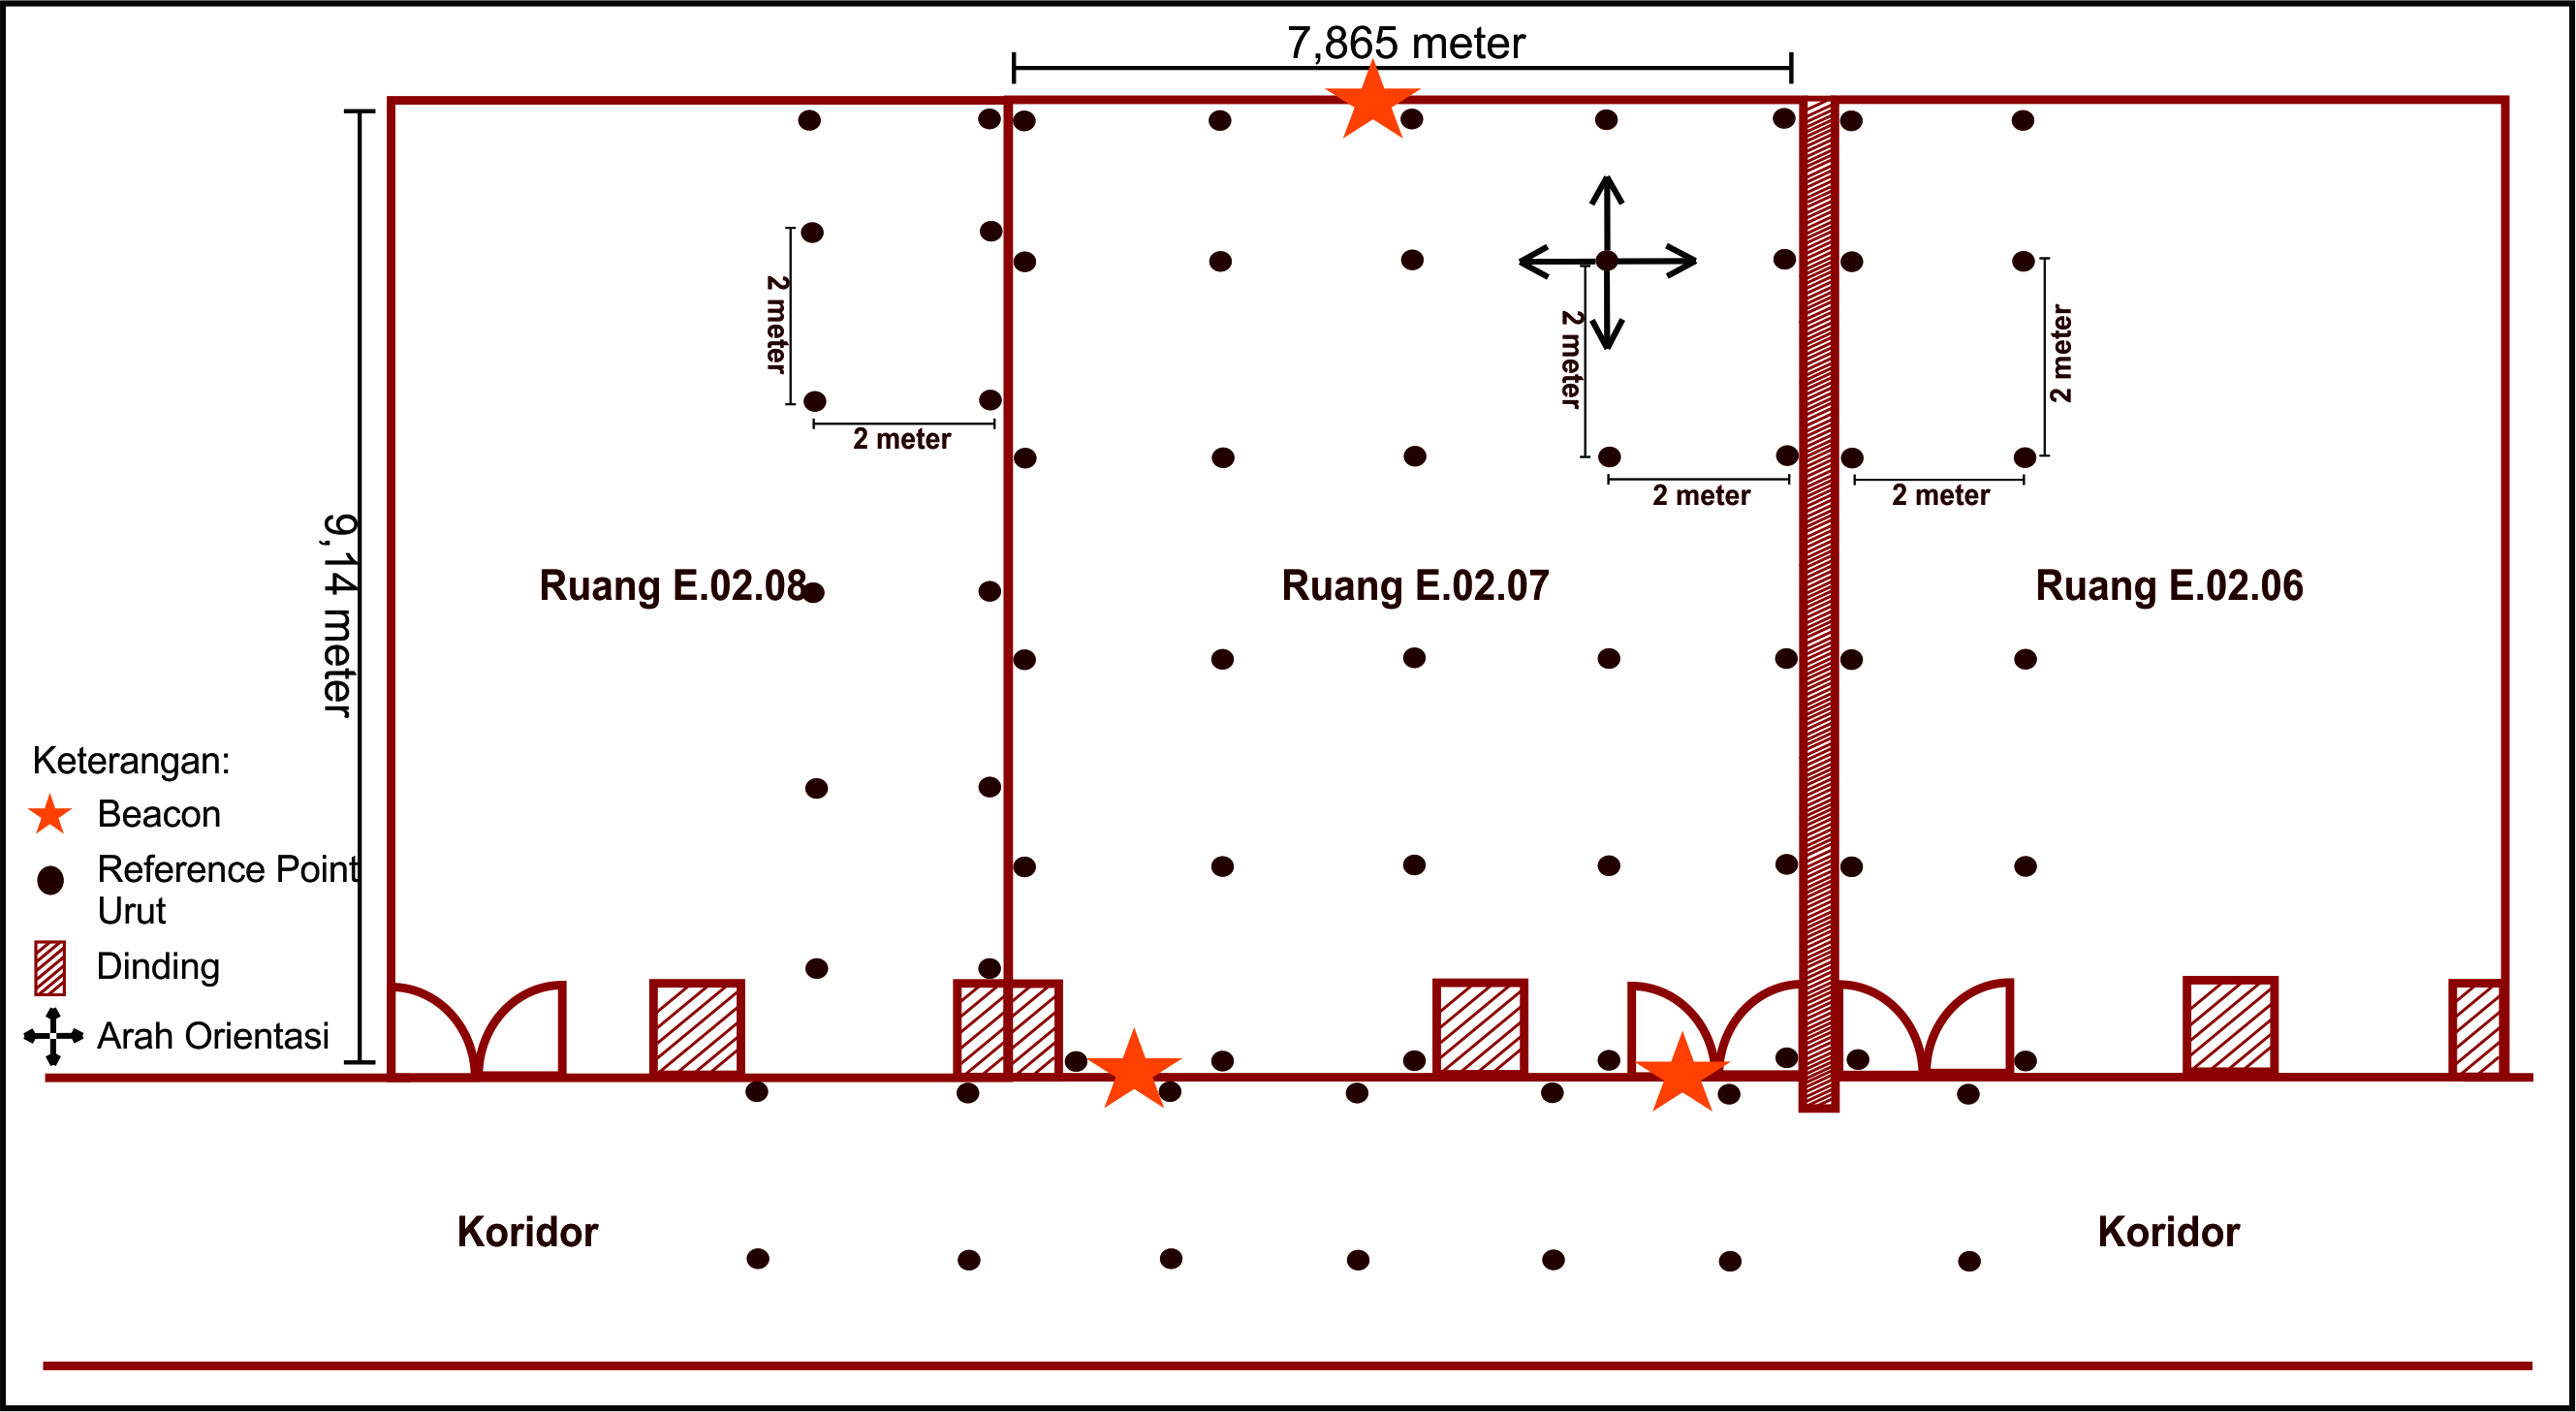
\includegraphics[width=13.3cm, height=8.2cm]{gambar/denah/E0207-Urut} }}%
    \qquad
    \\
    \subfloat[Reference Point Acak]{{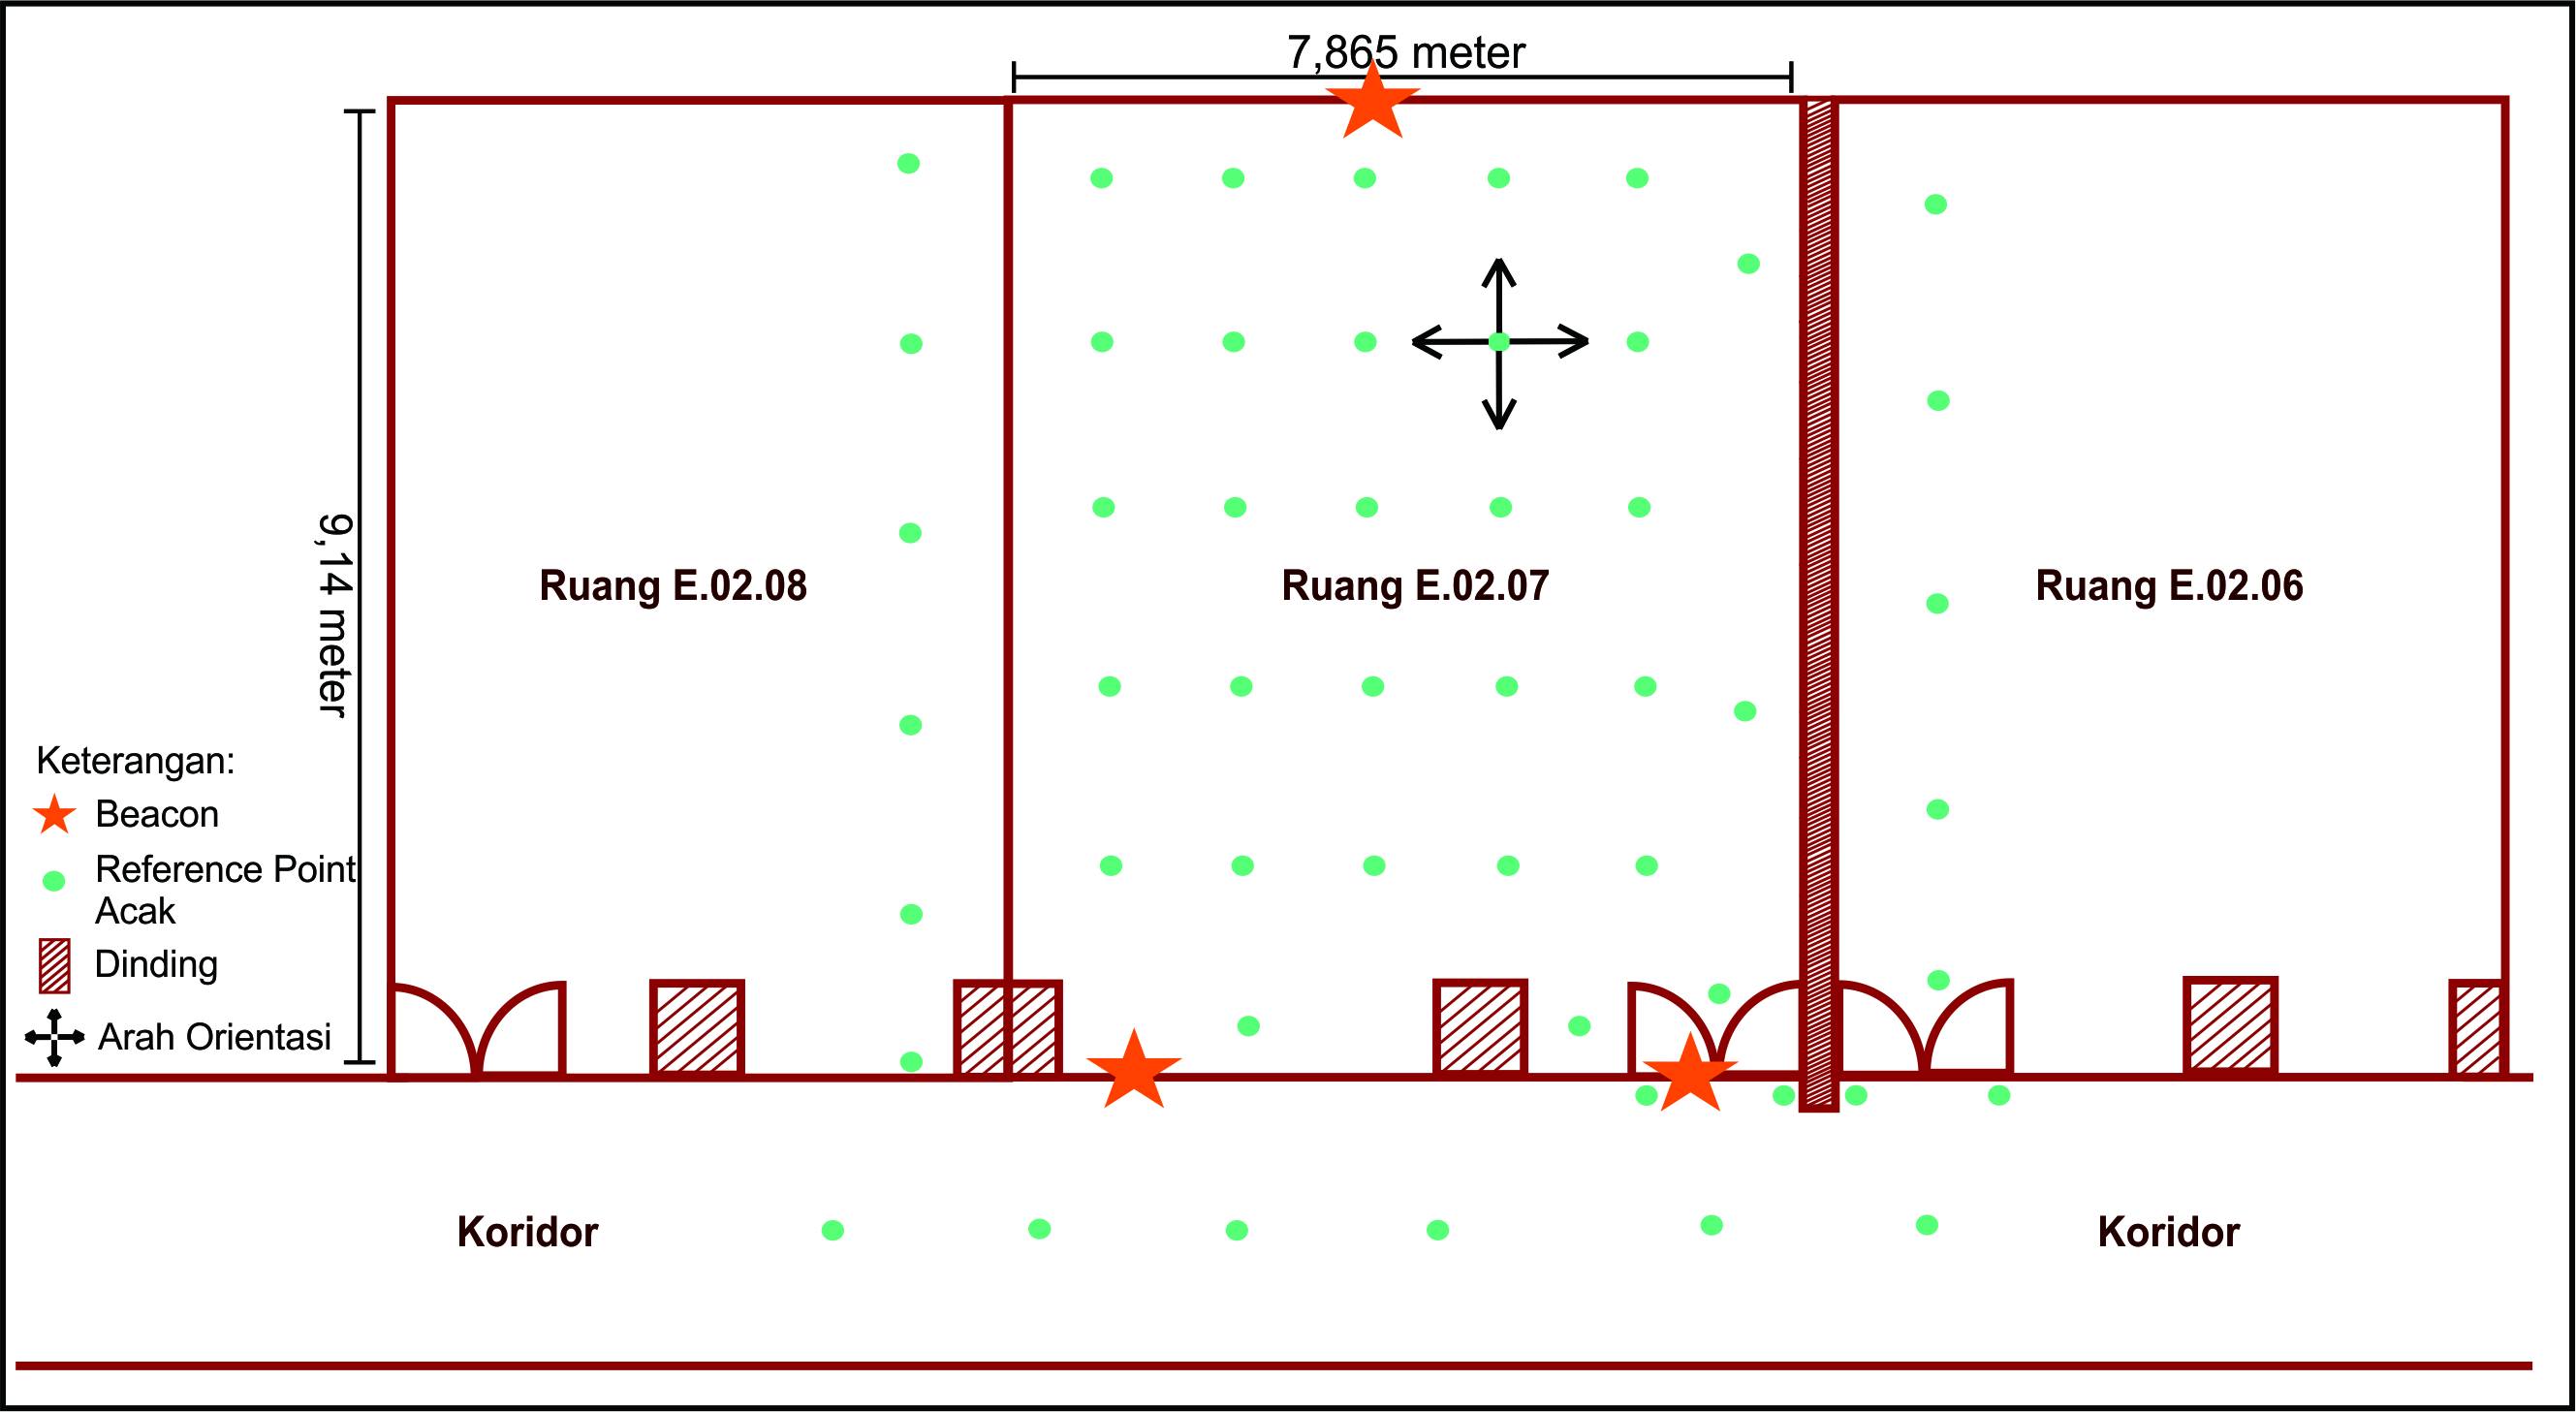
\includegraphics[width=13.3cm, height=8.2cm]{gambar/denah/E0207-Acak} }}%
    \caption{Denah Lokasi Penelitian Ruang E.02.07}%
    \label{kelase0207}%
\end{figure}

\par Proses pemetaan pengambilan kekuatan sinyal berdasarkan letak \textit{reference point} dilakukan dengan menghadap sebanyak 4 arah orientasi, yaitu: depan, kanan, belakang, dan kiri. Penelitian yang dilakukan oleh \cite{Bahl2000} menyebutkan bahwa kekuatan sinyal pada lokasi tertentu cukup bervariasi hingga -5 dBm tergantung pada arah yang dihadap pengguna. Dalam satu arah orientasi, antena \textit{host} yang dimiliki oleh \textit{smartphone} memiliki konektivitas \textit{line-of-sight} (LoS) ke sebuah antena Beacon selama orientasinya berlawanan. Arah orientasi dari tubuh pengguna juga dapat membentuk sebuah halangan dan kekuatan sinyal yang ditangkap juga berbeda. Oleh karena itu, perlu dilakukan pencatatan \textit{direction} (d), dengan menghadap ke depan, ke kanan, ke belakang dan ke kiri tergantung pada pengambilan kekuatan sinyal yang dilakukan \citep{christ1993}. Metode pengambilan kekuatan sinyal setiap Beacon berdasarkan proses survei pemetaan \textit{reference point} disebut dengan metode \textit{Fingerprinting}. Metode \textit{Fingerprinting} dilakukan dengan mengumpulkan dan menyimpan data-data kekuatan sinyal ke dalam basis data aplikasi untuk dijadikan sebagai data \textit{training}.  

%%%%%%%%%%%%%%%%%%%%%%next%%%%%%%%%%%%%%%%%%%%%
\item Pengumpulan Data \textit{Training}
\\
Pengumpulan data \textit {training} bertujuan untuk pembuatan basis data dari data kekuatan sinyal atau nilai RSSI yang didapat dari setiap Beacon. Pengumpulan data \textit{training} (\textit{offline}) dilakukan berdasarkan penentuan letak \textit{reference point} yang telah ditentukan sebelumnya. Pengumpulan data \textit{training} dengan pemetaan metode \textit{Fingerprinting} ini menggunakan Aplikasi Mapping yang telah dibuat dengan fitur-fitur untuk dapat menangkap kekuatan sinyal dari Beacon, kemudian informasi-informasi dari Beacon tersebut seperti MAC Address, nilai RSSI, dan nama ruangan dimana kekuatan sinyal tersebut ditangkap dapat disimpan pada aplikasi ini. Ilustrasi penyimpanan data \textit{training} dengan metode \textit{Fingerprinting} untuk \textit{reference point} urut dapat dilihat pada Tabel \ref{fingerprinting-sequence-point} dan untuk \textit{reference point} acak dapat dilihat pada Table \ref{fingerprinting-random-point}. Orientasi yang tercantum pada kedua gambar tersebut hanya sebagai gambaran bahwa penyimpanan data terhadap suatu posisi diambil berdasarkan 4 arah hadap.

\begin{landscape}
\begin{table}[H]
\caption{Ilustrasi Penyimpanan Data Training Metode \textit{Fingerprinting} pada \textit{Reference Point} Urut.}
\centering
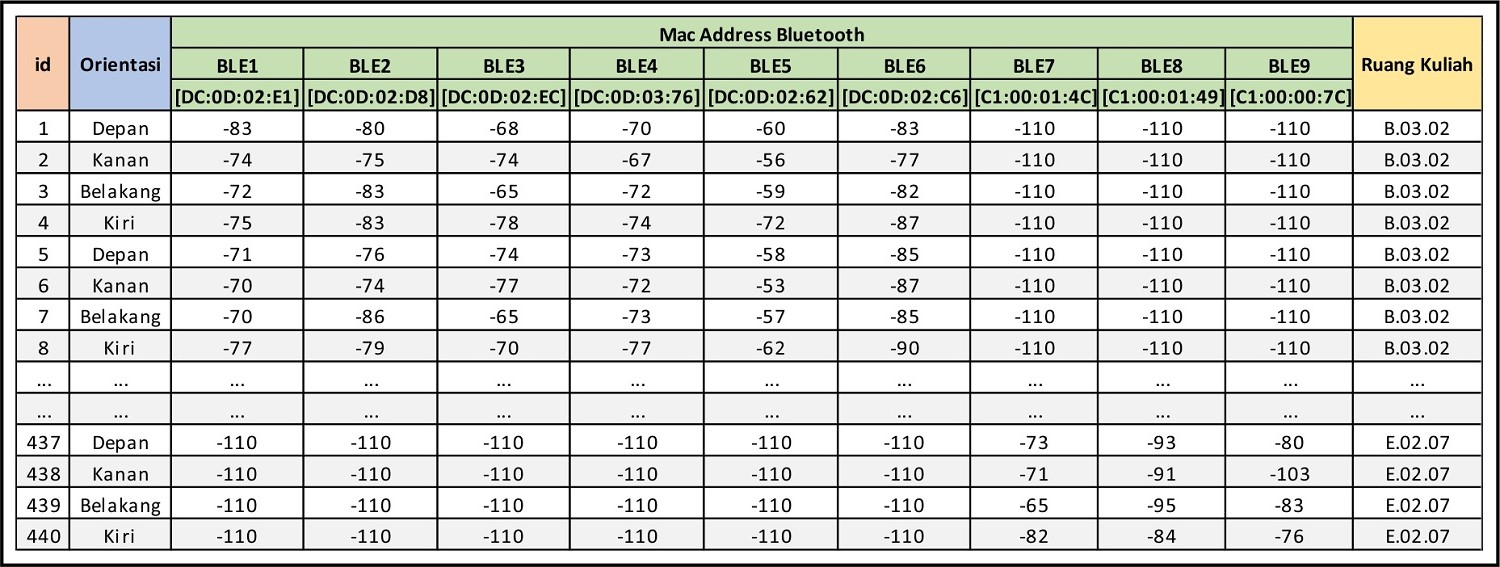
\includegraphics[width=20cm, height=9cm]{gambar/pengumpulan_data/sequence_point.jpg}
\label{fingerprinting-sequence-point}
\end{table}
\end{landscape}

\begin{landscape}
\begin{table}[H]
\caption{Ilustrasi Penyimpanan Data Training Metode \textit{Fingerprinting} pada \textit{Reference Point} Acak.}
\centering
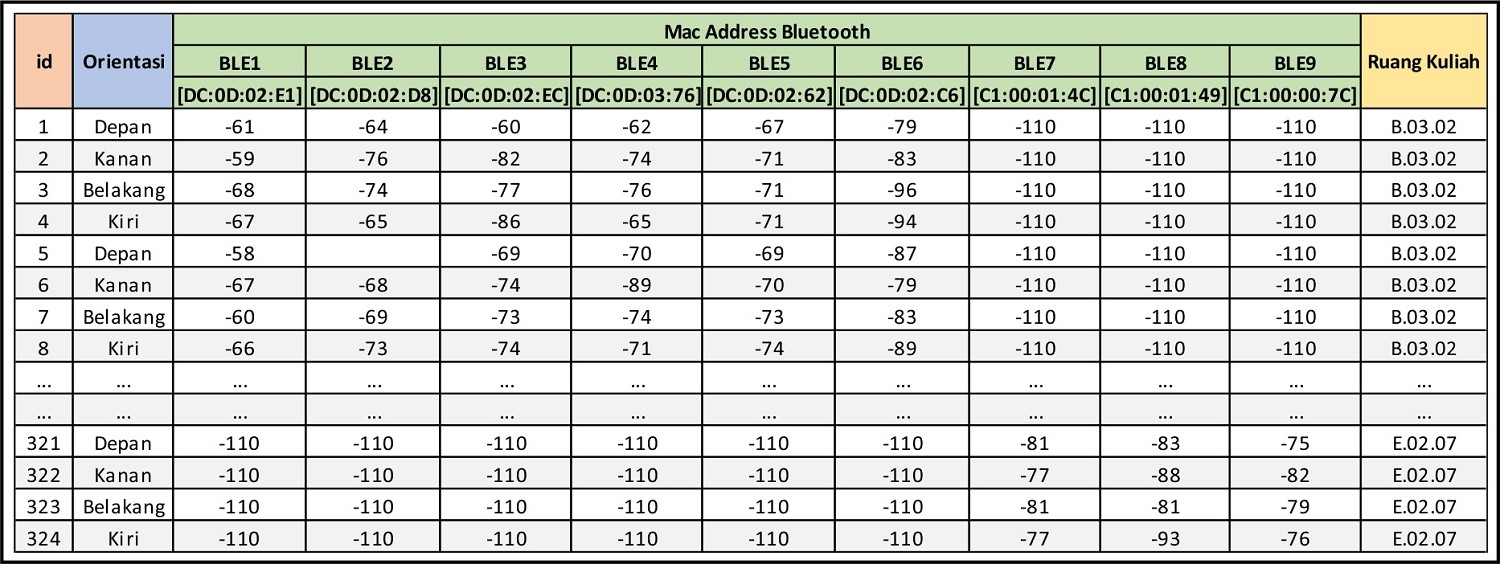
\includegraphics[width=20cm, height=9cm]{gambar/pengumpulan_data/random_point.jpg}
\label{fingerprinting-random-point}
\end{table}
\end{landscape}

\vspace{3cm}

\item Pengumpulan Data Uji
\\
Pengumpulan data uji bertujuan untuk menguji tingkat keberhasilan klasifikasi dengan melihat akurasi tertinggi bergantung pada parameter nilai \textit{k} yang digunakan. Pengumpulan data uji dilakukan setelah pengumpulan data \textit{training} dilakukan. Data uji bertindak seolah-olah kelas label belum diketahui. Data uji tersebut akan dibandingkan dengan data \textit{training} sebagai pengujian nilai \textit{k} terbaik, hasil dari nilai \textit{k} terbaik tersebut akan diimplementasikan pada Aplikasi Kehadiran Dosen dan Aplikasi Kehadiran Mahasiswa untuk memprediksi lokasi pengguna dengan metode klasifikasi K-NN.

\end{enumerate} 
%%%%%%%%%%%%%%%%%%%%%%%%%%%%%%%%%%%%%%%%%%%%%%%%%%%%%%%%%%%%%%%%%%%%%%%%%%%%%%%%%%%%%%%%%%%%%%%%%%%%%%%%%%%%%%%%%%%%%%%%%%%
%TESTING KNN%
\subsection{Pengujian Akurasi dengan Metode Klasifikasi K-NN}

\par Pengujian ini dilakukan dengan tujuan untuk mengetahui tingkat keberhasilan dari proses klasifikasi lokasi pengguna berdasarkan \textit{reference point} yang digunakan. Pengujian ini dilakukan dengan menggunakan parameter variasi nilai \textit{k} yang digunakan dalam penelitian ini, yaitu 3, 5 dan 7. Variasi nilai \textit{k} pada metode klasifikasi K-NN, digunakan untuk mencari nilai \textit{k} yang optimal sehingga tingkat akurasi tertinggi didapatkan. 

\par Proses klasifikasi yang diterapkan pada penelitian ini adalah analisa kuantitatif dengan membandingkan hasil perhitungan  nilai \textit{F-Measure} dari setiap parameter nilai \textit{k} yang ada. Parameter nilai \textit{k} terbaik ditentukan dari nilai \textit{F-Measure} terbesar dengan membandingkan parameter-parameter klasifikasi yang telah ditetapkan sebelumnya. Perhitungan nilai \textit{F-Measure} dilakukan berdasarkan hasil klasifikasi yang dapat dilihat pada Tabel \ref{tabel-matrix}.

\begin{table}[H]
\centering
\caption{Matriks Konfusi \citep{han2006}.}
\label{tabel-matrix}
\begin{tabular}{ccccl}
\cline{2-4}
\multicolumn{1}{c|}{}                                                                                      & \multicolumn{3}{c|}{\textbf{Diprediksi Sebagai}}                                                                      &  \\ \cline{1-4}
\multicolumn{1}{|c|}{\multirow{3}{*}{\textbf{\begin{tabular}[c]{@{}c@{}}Kelas\\ Sebenarnya\end{tabular}}}} & \multicolumn{1}{c|}{}                 & \multicolumn{1}{c|}{\textbf{Positif}} & \multicolumn{1}{c|}{\textbf{Negatif}} &  \\ \cline{2-4}
\multicolumn{1}{|c|}{}                                                                                     & \multicolumn{1}{c|}{\textbf{Positif}} & \multicolumn{1}{c|}{TP}               & \multicolumn{1}{c|}{FN}               &  \\ \cline{2-4}
\multicolumn{1}{|c|}{}                                                                                     & \multicolumn{1}{c|}{\textbf{Negatif}} & \multicolumn{1}{c|}{FP}               & \multicolumn{1}{c|}{TN}               &  \\ \cline{1-4}
\multicolumn{1}{l}{}                                                                                       & \multicolumn{1}{l}{}                  & \multicolumn{1}{l}{}                  & \multicolumn{1}{l}{}                  & 
\end{tabular}
\end{table}
Keterangan:\newline
$TP$ = \textit{True} Positif. \newline
$FP$ = \textit{False} Positif. \newline
$FN$ = \textit{False} Negatif. \newline
$TN$ = \textit{True} Negatif. \newline
\par Tabel \ref{tabel-matrix} merepresentasikan prediksi dan kelas sebenarnya, sehingga dapat digunakan untuk menentukan \textit{precision}, \textit{recall}, dan \textit{F-Measure}. \textit{Precision} ($p$) merupakan perbandingan antara data yang benar diklasifikasikan positif dengan total data yang diklasifikasikan positif yang dapat dilihat dengan rumus: 

\begin{equation}
p= \frac{TP} {TP+FP}
\end{equation}
%end precision

\par Recall ($r$) merupakan perbandingan antara data yang benar diklasifikasikan positif dengan total data yang seharusnya positif yang dapat dilihat dengan rumus:

\begin{equation}
r= \frac{TP} {TP+FN} 
\end{equation}
\newline
\par Rumus untuk menghitung \textit{F-Measure} $(F)$ adalah sebagai berikut:

\begin{equation}
F=2 \cdot \frac{p.r} {p+r}
\end{equation}
\newline
Keterangan:\newline
$p$ = \textit{precision}. \newline
$r$ = \textit{recall}. 

\subsection{Pembuatan Aplikasi Kehadiran dan Aplikasi Web Admin}
\begin{enumerate}

\item Aplikasi Kehadiran Dosen
\newline
Aplikasi ini merupakan aplikasi \textit{mobile} berbasis Android yang berguna untuk mempermudah dosen melakukan proses pencatatan kehadiran perkuliahan di Jurusan Informatika Unsyiah, yang dikembangkan dengan konsep \textit{Indoor Positioning System}. Aplikasi ini bekerja apabila perangkat \textit{smartphone} sudah mendukung Bluetooth 4.0, dikarenakan aplikasi ini menangkap kekuatan sinyal atau nilai RSSI dari Beacon yang terintegrasi BLE di dalamnya. Kekuatan sinyal yang ditangkap akan dilakukan perhitungan menggunakan metode klasifikasi K-NN, \textit{output} dari perhitungan tersebut adalah prediksi lokasi dosen yang akan dikirim ke \textit{web services} secara \textit{background process} sebagai bukti kehadiran. Adapun fitur-fitur yang tersedia adalah sebagai berikut:

\begin {itemize}
\itemsep0em
\item Memproses Pencatatan Data Kehadiran \newline
Pada aplikasi ini, dosen diwajibkan untuk memulai proses pencatatan data kehadiran perkuliahan dengan menekan tombol \textbf{start attendance}. Proses pencatatan data kehadiran perkuliahan dapat dimulai apabila sudah pada waktunya dan tidak dapat dimulai apabila dosen sudah terlambat selama 50 menit. Aplikasi akan memproses kehadiran dosen sampai mata kuliah berakhir.

\item Menampilkan Jadwal Perkuliahan \newline
Aplikasi dapat menampilkan jadwal perkuliahan yang dimiliki oleh masing-masing dosen per-harinya. Apabila dosen menekan salah satu jadwal perkuliahan, akan diarahkan ke halaman informasi mata kuliah tersebut seperti: kode mata kuliah, nama mata kuliah, waktu perkuliahan, nama ruangan, dan jumlah mahasiswa yang mengambil mata kuliah.

\item Melihat Daftar Mahasiswa \newline
Aplikasi ini menyediakan fitur agar dosen dapat melihat daftar nama mahasiswa yang mengambil suatu mata kuliah. 

\end{itemize}

\item Aplikasi Kehadiran Mahasiswa
\newline
Aplikasi ini merupakan aplikasi \textit{mobile} berbasis Android yang berguna untuk mempermudah mahasiswa melakukan proses pencatatan kehadiran perkuliahan di Jurusan Informatika Unsyiah, yang dikembangkan dengan konsep \textit{Indoor Positioning System}. Aplikasi ini bekerja apabila perangkat \textit{smartphone} sudah mendukung Bluetooth 4.0, dikarenakan aplikasi ini menangkap kekuatan sinyal atau nilai RSSI dari Beacon yang terintegrasi BLE di dalamnya. Kekuatan sinyal yang ditangkap akan dilakukan perhitungan menggunakan metode klasifikasi K-NN, \textit{output} dari perhitungan tersebut adalah prediksi lokasi mahasiswa yang akan dikirim ke \textit{web services} secara \textit{background process} sebagai bukti kehadiran. Adapun fitur-fitur yang tersedia adalah sebagai berikut:
 
\begin {itemize}
\itemsep0em
\item Memproses Pencatatan Data Kehadiran \newline
Mahasiswa dapat memulai proses pencatatan data kehadiran apabila dosen sudah memulai perkuliahan. Aplikasi akan memproses pencatatan data kehadiran mahasiswa sampai mata kuliah berakhir.

\item Menampilkan Jadwal Perkuliahan \newline
Aplikasi memiliki fitur untuk menampilkan jadwal perkuliahan yang dimiliki oleh masing-masing mahasiswa per-harinya. Jadwal perkuliahan yang ditampilkan berisi informasi seperti: nama dosen yang mengajar, kode mata kuliah, nama mata kuliah, ruangan, dan waktu perkuliahan.

\item Melihat Mata Kuliah \newline
Pada aplikasi ini, mahasiswa dapat melihat daftar mata kuliah yang diambil pada sistem KRS Online. Aplikasi menampilkan informasi-informasi setiap mata kuliah tersebut.
\end{itemize}

\item Aplikasi Rekap Kehadiran Mahasiswa dan Kehadiran Dosen
\newline
Aplikasi ini merupakan aplikasi berbasis web yang berguna untuk mempermudah staf dan admin untuk merekap data kehadiran dosen dan mahasiswa di Jurusan Informatika Unsyiah. Aplikasi ini menyajikan data daftar kehadiran dosen dan mahasiswa berdasarkan pada kode mata kuliah dan tanggal pelaksanaan perkuliahan yang dipilih. Aplikasi ini dapat mengunduh data rekapitulasi daftar kehadiran dosen dan mahasiswa ke dalam bentuk format CSV. 

\end{enumerate}
%%%%%%%%%%%%%%%%%%%%%%%%%%%%%%%%%%%%%%%%%%%%%%%%%%%%%%%%%%%%%%%%%%%%%%%%%%%%%%%%%%%%%%%%%%%%%%%%%%%%%%%%%%%%%%%%%%%%%%%%%%%%%%%
\subsection{Pengujian Fungsionalitas dengan Metode Black Box}
\par Pengujian \textit{Black Box} berfokus pada spesifikasi fungsionalitas dari sistem yang telah dibuat dengan mengeksekusi dan menjalankan sistem tersebut apakah sesuai dengan alur bisnis yang diinginkan. Pengujian ini melihat fungsi yang tidak sesuai pada sistem, kesalahan-kesalahan sistem dalam mengerjakan suatu perintah, dan kesalahan-kesalahan pada struktur data dan akses basis data. 

\subsection{Pengujian Usabilitas dengan Metode SUS}
\par Salah satu prinsip utama yang dijadikan sebagian tolak ukur keberhasilan dari pengembangan perangkat lunak adalah nilai pengujian itu sendiri. \textit{Usability Testing} dilakukan untuk melihat dan mengevaluasi sebuah produk atau jasa dengan cara menguji kepada calon pengguna dengan menggunakan metode SUS. SUS terdiri dari 10 pertanyaan dengan menggunakan skala likert 1-5. Berikut daftar pertanyaan-pertanyaan metode SUS dapat dilihat pada Tabel \ref{tabel-pertanyaan-sus}.  
%TABEL PERTANYAAN SUS%
\begin{table}[H]
\center
\caption{Daftar Pertanyaan Metode SUS \citep{Sharfina2016}}
\label{tabel-pertanyaan-sus}
\begin{tabular}{|c|l|l}
\cline{1-2}
\textbf{\begin{tabular}[c]{@{}c@{}}Kode \\ Pertanyaan\end{tabular}} & \multicolumn{1}{c|}{\textbf{Daftar Pertanyaan}}                                                                               &  \\ \cline{1-2}
$R1$                                                                  & Saya berpikir akan menggunakan sistem ini                                                                                     &  \\ \cline{1-2}
$R2$                                                                  & Saya merasa sistem ini sulit untuk digunakan                                                                                  &  \\ \cline{1-2}
$R3$                                                                  & Saya merasa sistem ini mudah digunakan                                                                                        &  \\ \cline{1-2}
$R4$                                                                  & \begin{tabular}[c]{@{}l@{}}Saya akan membutuhkan bantuan orang lain \\ untuk menggunakan sistem ini\end{tabular}              &  \\ \cline{1-2}
$R5$                                                                  & \begin{tabular}[c]{@{}l@{}}Saya merasa fitur-fitur pada sistem ini sudah \\ berjalan dengan sebagaimana mestinya\end{tabular} &  \\ \cline{1-2}
$R6$                                                                  & \begin{tabular}[c]{@{}l@{}}Saya merasa banyak hal-hal yang tidak \\ konsisten (tidak serasi) pada sistem ini\end{tabular}     &  \\ \cline{1-2}
$R7$                                                                  & \begin{tabular}[c]{@{}l@{}}Saya merasa orang lain dapat memahami cara\\ menggunakan aplikasi ini dengan cepat\end{tabular}    &  \\ \cline{1-2}
$R8$                                                                  & Saya merasa aplikasi ini membingungkan                                                                                        &  \\ \cline{1-2}
$R9$                                                                  & \begin{tabular}[c]{@{}l@{}}Saya merasa nyaman (tidak ada hambatan) \\ dalam menggunakan sistem ini\end{tabular}               &  \\ \cline{1-2}
$R10$                                                                 & \begin{tabular}[c]{@{}l@{}}Saya perlu membiasakan diri terlebih dahulu \\ sebelum menggunakan aplikasi ini\end{tabular}       &  \\ \cline{1-2}
\end{tabular}
\end{table}

\par Rumus untuk menghitung skor akhir metode SUS \citep{Brooke1996}, dapat dilihat dari persamaan berikut.
\begin{equation}
skorSUS = (\sum_{9}^{i} (Ri - 1) + \sum_{10}^{j} (5 - Rj)) * 2,5
\end{equation}
\newline
Keterangan:\newline
$R$ = daftar pertanyaan pada metode SUS. \newline
$i$ = angka ganjil 1, 3, 5, 7, dan 9. \newline
$j$ = angka genap 2, 4, 6, 8, dan 10.
\newline 

\par Tingkat nilai skala pengujian menentukan apakah sistem tersebut layak digunakan, bermanfaat, diterima oleh \textit{user} dan bertahan lama penggunaannya. Sebuah sistem dengan nilai pengujian yang tinggi membuat sistem tersebut menjadi populer dalam waktu yang lama dan penggunaannya yang luas, karena banyak individu akan merasakan manfaat dari kehadiran sistem tersebut. Sedangkan sistem dengan nilai pengujian yang rendah, seringkali diabaikan oleh pengguna walaupun dibuat berdasarkan kebutuhan dan menghasilkan sumber daya yang banyak. Berdasarkan dari skor akhir SUS tersebut, dapat diketahui bahwa seberapa tinggi tingkat \textit{usability} rancangan sistem yang dikembangkan. Tabel \ref{tabelsus} menunjukkan nilai interpretasi yang digunakan.

\begin{table}[H]
\center
\caption{Interpretasi skor SUS \citep{Bangoor2009}.}
\label{tabelsus}
\begin{tabular}{|c|c|lll}
\cline{1-2}
\textbf{Skor SUS} & \textbf{Interprestasi} &  &  &  \\ \cline{1-2}
\textless{}50     & Tidak Dapat Diterima   &  &  &  \\ \cline{1-2}
50-70             & Marginal               &  &  &  \\ \cline{1-2}
\textgreater{}70  & Dapat Diterima         &  &  &  \\ \cline{1-2}
\end{tabular}
\end{table}

%%%%%%%%%%%%%%%%%%%%%%%%%%%%%%%%%%%%%%%%%%%%%%%%%%%%%%%%%%%%%%%%%%%%%%%%%%%%%%%%%%%%%%%%%%%%%%%%%%%%%%%%%%%%%%%%
\subsection{Analisis Keakuratan}
Penelitian ini memiliki dua analisis keakuratan dalam penentuan lokasi pengguna. Analisis keakuratannya adalah sebagai berikut:
\begin{enumerate}[1.]
\item Membandingkan tingkat keakuratan klasifikasi antara \textit{reference point} urut dan \textit{reference point} acak.
\item Membandingkan tingkat keakuratan dalam memprediksi lokasi pengguna menggunakan jumlah Beacon yang berbeda, yaitu dengan jumlah 3 Beacon dan 6 Beacon.
\end{enumerate}
